\documentclass{beamer}

\usepackage{mpemath}
\usepackage{subcaption}
\usepackage[normalem]{ulem}
\usepackage{amsmath}
\usepackage{amssymb}
\usepackage{mathtools}
%\usepackage{pgf}
%\usepackage{pgfplots}
%\usepackage{tikz}
\usepackage{booktabs}
\usepackage{siunitx}
\usepackage{natbib}
\usepackage{tabularx}
\usepackage{multirow}
\usepackage{amsmath}
\usepackage{mathtools}
\usepackage{amssymb}
\usepackage{bbm}
\usepackage[dvipsnames]{xcolor} % Saved my life during a conference once


%\usetikzlibrary{arrows,automata,backgrounds,positioning,decorations,intersections,matrix}

% *** Styles ***
\usetheme{Singapore}
\setbeamertemplate{navigation symbols}{}
% \usetheme[progressbar=frametitle]{metropolis}
% \usecolortheme{dolphin}
%\useinnertheme{circles}
%\usecolortheme{rose}
%\setbeamercovered{transparent}
\setbeamercovered{invisible}
\usefonttheme{professionalfonts}
%\usefonttheme[onlymath]{serif}
\setbeamertemplate{footline}[frame number]

\title{Mitigating the Curse of Horizon in Monte-Carlo Returns}
\author{Gersi Doko}
\institute{Department of Computer Science \\ University of New Hampshire}
\date{}

\AtBeginSection[]{
	\begin{frame}
          \vfill
	\centering
	% \usebeamerfont{title}
        {\huge\bf \insertsectionhead}%
	\vfill
\end{frame}
}

\begin{document}

\frame{\titlepage}

\section*{Intro}

\begin{frame}
\frametitle{Financial Analysts}
  \vfill
  \emph{Goal: }We want $\mathcal{R} : \tilde{X} \to \Real$ that represents the "hazard" for $\tilde{X} : \Omega \to \Real$
  \vfill
\end{frame}

\begin{frame}
\frametitle{Insurance Providers}
  \vfill
  \emph{Goal: }We want $\mathcal{D} : \tilde{X} \to \Real$ that represents the "uncertainty" for $\tilde{X} : \Omega \to \Real$
  \vfill
\end{frame}

\begin{frame}
\frametitle{ML Practitioners}
  \vfill
  \emph{Goal: }We want $\mathcal{E} : \tilde{X} \to \Real$ that represents the "non-zeroness" for $\tilde{X} : \Omega \to \Real$
  \vfill
\end{frame}

\begin{frame}
\frametitle{Risk Quadrangle}
  \vfill
  \emph{Goal: }We want $\mathcal{R} : \tilde{X} \to \Real$ that represents the "hazard" for $\tilde{X} : \Omega \to \Real$
  \vfill
  \emph{Goal: }We want $\mathcal{D} : \tilde{X} \to \Real$ that represents the "uncertainty" for $\tilde{X} : \Omega \to \Real$
  \vfill
  \emph{Goal: }We want $\mathcal{E} : \tilde{X} \to \Real$ that represents the "non-zeroness" for $\tilde{X} : \Omega \to \Real$
  \vfill
  \textbf{Observation:  The three goals are not independent}
\end{frame}

\begin{frame}
	\frametitle{Risk Quadrangle}
  \vfill
  \begin{figure}[ht]
    \centering
    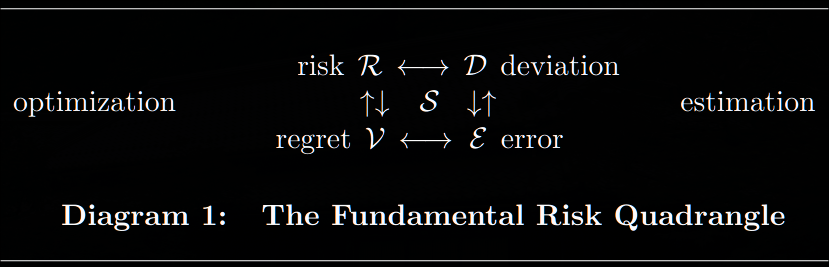
\includegraphics[width=\textwidth]{./imgs/risk_quadrangle.png}
  \end{figure}
  \vfill
\end{frame}
\begin{frame}
	\frametitle{Risk Quadrangle}
  \vfill
  \begin{figure}[ht]
    \centering
    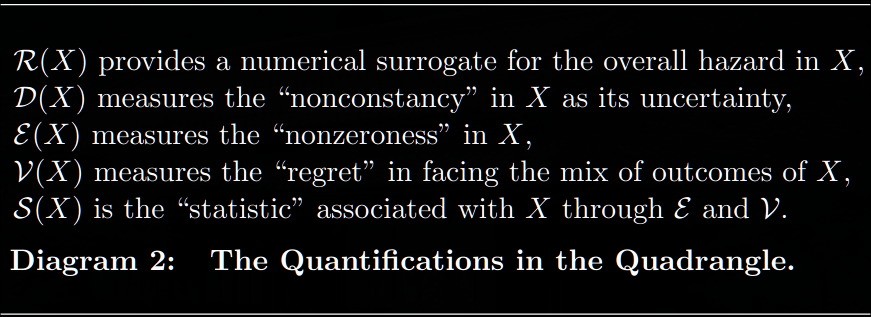
\includegraphics[width=\textwidth]{./imgs/riskquaddesc.png}
  \end{figure}
  \vfill
\end{frame}

\begin{frame}
\frametitle{Risk Quadrangle}
  \vfill
  \emph{Today:} we focus on what relates all of these measures
  \vfill
\end{frame}

\begin{frame}
  \frametitle{$\mathcal{R}(\tilde{X})$}
  \vfill
  How should we give meaning to the statement
  $$\tilde{X} \text{ "adequately" }\leq C$$
  \vfill
  $$\mathbb{E}(\tilde{X}) \leq C$$
  $$\mathbb{E}(\tilde{X}) + \lambda \sigma(\tilde{X}) \leq C$$
  $$q_\alpha(\tilde{X}) \leq C$$
  $$\sup(\tilde{X}) \leq C$$
\end{frame}

\begin{frame}
  \frametitle{$\mathcal{D}(\tilde{X})$}
  \vfill
  How should we give meaning to the statement
  $$\tilde{X} \text{ "adequately" }\leq C$$
  \vfill
  $$\mathbb{E}(\tilde{X}) \leq C$$
  $$\mathbb{E}(\tilde{X}) + \lambda \sigma(\tilde{X}) \leq C$$
  $$q_\alpha(\tilde{X}) \leq C$$
  $$\sup(\tilde{X}) \leq C$$
\end{frame}


\end{document} 
